\documentclass{article}
\usepackage[margin=1in]{geometry}
\usepackage{fancyvrb,graphicx,hyperref}
\title{CSCI 241, Spring 2017, Project \#1}
\author{Geoffrey Matthews}
\begin{document}
\maketitle

\centerline{\bf NOTE:  this is incomplete.}

\begin{description}
\item[Due date:]  April 28, midnight.

\item[Turn in:] Be sure to {\bf zip} all your source files together
  before submission.  Canvas downloads mangle the names, and java
  likes to have the names of the files the same as the public class in
  the file.

  To make
  it easier for me to write scripts to unpack, compile, and run your
  file:
  \begin{itemize}
    \item
      Use {\bf zip}, not tar or 7z or any other archiving software.
      \item Zip the folder, not the individual  files in the folder.
      \item Name the zip file {\tt lab01.zip}.
\item
  Nmae the file (and class) with your {\tt main} method in it {\tt
    lab01.java}. 
  \end{itemize}
  
\item[Caesar ciphers:]

  \begin{figure}
  \centerline{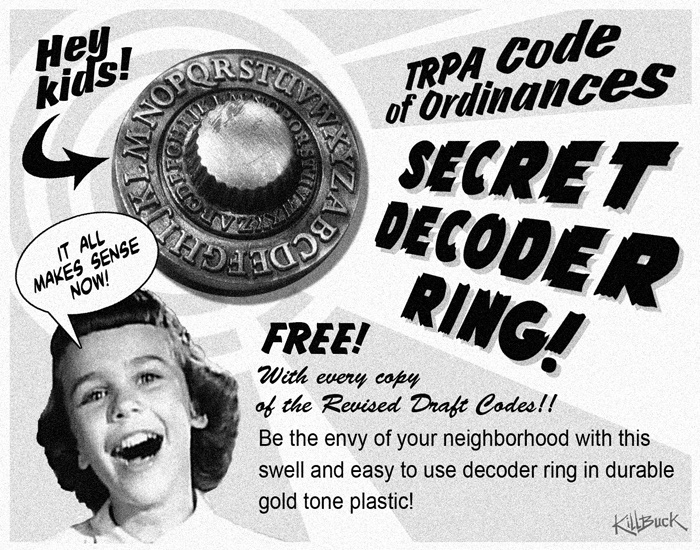
\includegraphics[scale=0.25]{secretdecoderring.jpg}  }
  \caption{Magic decoder ring.}
  \label{magicring}
  \end{figure}
  
Caesar ciphers are a simple way of enciphering messages and form the
basis of the secret decoder ring (see Figure \ref{magicring}).  A
shift of the alphabet is used.  For example, a shift of 3 (or,
equivalently, shift to ``D'') gives the following table:

\hspace{-0.5in}\mbox{
\begin{tabular}{|c|c|c|c|c|c|c|c|c|c|c|c|c|c|c|c|c|c|c|c|c|c|c|c|c|c|}\hline
A&B&C&D&E&F&G&H&I&J&K&L&M&N&O&P&Q&R&S&T&U&V&W&X&Y&Z\\\hline
D&E&F&G&H&I&J&K&L&M&N&O&P&Q&R&S&T&U&V&W&X&Y&Z&A&B&C\\\hline
\end{tabular}
}

To encipher a letter, look it up in the top row, but use the letter in
the bottom row.  For example, ``HELLO WORLD'' becomes ``KHOOR ARUOG''
(Klingon, I think).

To decipher a message enciphered with a Caesar cipher, you need to
find the {\em key}, a number between 0 and 25 (or a letter between
``A'' and ``Z'').  Since there are only 26 Caesar ciphers, it would be
easy to just try them all to break a message enciphered with one.  But
we need a little more sophistication for what follows.

Instead, we rely on {\em frequency analysis}.  English text is not
uniformly distributed among all 26 letters.  ``E'', for instance, is
much more common than ``Q''.  If you take a large body of English text
and count the occurrences of each letter, you get a distribution like
that in Figure \ref{letterfrequencies}.  There are clear patterns in
the frequencies.  E, for example, occurs quite a bit more frequently
than any other letter.  Further, the sequential letters UVWXYZ are all
fairly infrequent, and so they create a noticeable ``trough'' of five
sequential letters. 

\begin{figure}
  \begin{center}
    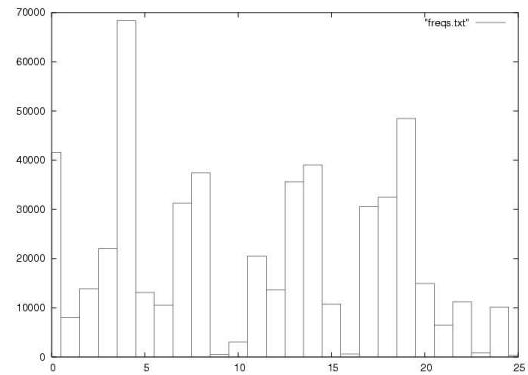
\includegraphics[scale=0.5]{freqhist01.png}
  \end{center}
  \caption{Letter frequencies for English.}
  \label{letterfrequencies}
\end{figure}

\begin{figure}
  \begin{center}
    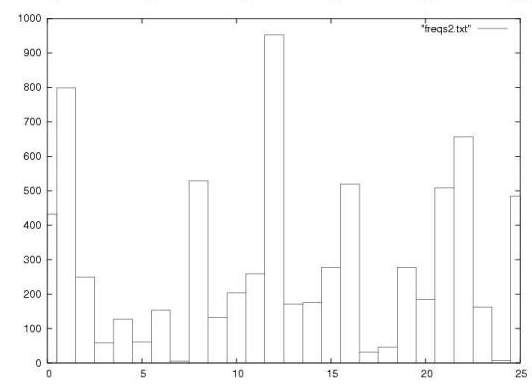
\includegraphics[scale=0.5]{freqhist02.png}
  \end{center}
  \caption{Letter frequencies for Caesar enciphered English.}
  \label{encipheredfrequencies}
\end{figure}

If you take any other work in English that has been enciphered with a
Caesar cipher, and look at the letter frequencies, you will get
something similar to Figure \ref{encipheredfrequencies}.  The
histograms are not exactly the same, but you can see the same
patterns.  The highest one is probably E.  There is also a trough of
five sequential letters, probably UVWXYZ, and its position relative to
the supposed E is appropriate.  We can be fairly confident that the
key to this Caesar cipher is a shift of 8.

\item[Vigenere ciphers:]  Caesar ciphers are so easy to break that it
  is doubtful they were ever used (even by Caesar) to encipher
  important information.  However, they form the basis for a much more
  sophisticated cipher that has been used:  Vigenere square ciphers.

Vigenere squares were once thought to be unbreakable.  It was Charles
Babbage (the guy who invented the computer) who figured out how to
break them (even without a computer).

Here's how they work.  Let's suppose that we have a procedure to
encipher with Caesar ciphers, {\tt encipher(letter, key)} will
encipher the character {\tt letter} with the Caesar cipher with key {\tt
  key}.  Then (consulting the table above), {\tt encipher('M', 'D') =>
  'P'}, for example.  Note that {\tt encipher(x,y) == encipher(y,x)}.

We can now encipher a long text and break up the frequencies of the
output letters by using a different Caesar cipher for different
letters in the text.  Instead of a key being a single letter, a key is
now a {\em keyword}.  The letters of the keyword (repeated as
necessary) tell us which Caesar cipher to use for each letter in the
input.

For example, suppose the keyword is ``fumble'' and the plaintext is
``meet me at midnight.''  Then we encipher the message as
follows:

\begin{tabular}{|c|c|c|c|c|c|c|c|c|c|c|c|c|c|c|c|c|}
    \hline
  Plaintext: &  M&E&E&T&M&E&A&T&M&I&D&N&I&G&H&T  \\\hline
  Keyword: &    F&U&M&B&L&E&F&U&M&B&L&E&F&U&M&B  \\\hline
  Ciphertext: & R&Y&Q&U&X&I&F&N&Y&J&O&R&N&A&T&U  \\\hline
\end{tabular}

Thus, we use {\tt encipher('M', 'F')}, {\tt encipher('E', 'U')},
{\tt encipher('E', 'M')}, {\em etc.} as the ciphertext.

Letter frequencies and patterns are completely broken up with this
strategy.  For example, the double-e (a common pattern in English) in
``meet'' is {\em not} enciphered by a double letter.  Further, since
Es in general are enciphered by several different keys into several
different letters, pretty much at random, and further since other
letters will also be enciphered into the same letters that E is using,
no one of encipherings of E will dominate and no one letter in the
ciphertext will have a much larger frequency than the others.

\item[A Vigenere Square:]  Historically, this cipher would have been
  used without computers, by a spy hiding in a closet with few
  materials. If all he or she knew was the keyword, they could still
  construct everything they needed quickly.  A Vigenere square, such
  as the one in Figure \ref{vigeneresquare}, can be constructed by
  hand very quickly.  Then you simply use the plaintext letter and the
  cipher key as the row and column to lookup your ciphertext letter. 

A ruler or other straightedge would obviously be a big help.

  \begin{figure}

{\small
\begin{Verbatim}
                A B C D E F G H I J K L M N O P Q R S T U V W X Y Z
                B C D E F G H I J K L M N O P Q R S T U V W X Y Z A 
                C D E F G H I J K L M N O P Q R S T U V W X Y Z A B 
                D E F G H I J K L M N O P Q R S T U V W X Y Z A B C 
                E F G H I J K L M N O P Q R S T U V W X Y Z A B C D 
                F G H I J K L M N O P Q R S T U V W X Y Z A B C D E 
                G H I J K L M N O P Q R S T U V W X Y Z A B C D E F 
                H I J K L M N O P Q R S T U V W X Y Z A B C D E F G 
                I J K L M N O P Q R S T U V W X Y Z A B C D E F G H 
                J K L M N O P Q R S T U V W X Y Z A B C D E F G H I 
                K L M N O P Q R S T U V W X Y Z A B C D E F G H I J 
                L M N O P Q R S T U V W X Y Z A B C D E F G H I J K 
                M N O P Q R S T U V W X Y Z A B C D E F G H I J K L 
                N O P Q R S T U V W X Y Z A B C D E F G H I J K L M 
                O P Q R S T U V W X Y Z A B C D E F G H I J K L M N 
                P Q R S T U V W X Y Z A B C D E F G H I J K L M N O 
                Q R S T U V W X Y Z A B C D E F G H I J K L M N O P 
                R S T U V W X Y Z A B C D E F G H I J K L M N O P Q 
                S T U V W X Y Z A B C D E F G H I J K L M N O P Q R 
                T U V W X Y Z A B C D E F G H I J K L M N O P Q R S 
                U V W X Y Z A B C D E F G H I J K L M N O P Q R S T 
                V W X Y Z A B C D E F G H I J K L M N O P Q R S T U 
                W X Y Z A B C D E F G H I J K L M N O P Q R S T U V 
                X Y Z A B C D E F G H I J K L M N O P Q R S T U V W 
                Y Z A B C D E F G H I J K L M N O P Q R S T U V W X
                Z A B C D E F G H I J K L M N O P Q R S T U V W X Y
\end{Verbatim}
}      

\caption{A Vigenere Square.}
\label{vigeneresquare}
\end{figure}

\item[Breaking Vigenere ciphers:]  What Charles Babbage realized,
  however, was that a Vigenere cipher is just $n$ Caesar ciphers,
  where $n$ is the length of the keyword, usually not very large.  If
  we can guess the length of the keyword somehow, we can break the
  Vigenere ciphertext into $n$ Caesar ciphertexts, and break each of
  them with frequency counts.  

  How do we guess the length of the keyword?  If we have a longish
  ciphertext, and a relatively short keyword (the norm for
  human-generated ciphers), there are bound to be
  places where a common English word, like ``the,'' (or even a common
  {\em phrases} of English such as ``on the'' or ``in the'' or ``when
  the'') lines up with the keyword at the same spot.  For example,
  with the keyword ``fumble,'' you are likely to have this kind of
  thing happen:

  \begin{tabular}{|r|c|c|c|c|c|c|c|c|c|}\hline
Plaintext: &    ... & T & H & E & ... & T & H & E & ...\\\hline
Keyword: &      ... & M & B & L & ... & M & B & L & ...\\\hline
Ciphertext: &   ... & F & I & P & ... & F & I & P & ...\\\hline
\end{tabular}


Note two things about this phenomenon: First, the ciphertext is
identical.  Second, the distance between the identical substrings must
be a multiple of the length of the keyword.

The second fact must be 
true about virtually every pair of identical substrings in the
ciphertext.  Even a fairly short pair of identical substrings is
unlikely to happen by accident. (What are the odds of a length-5
substring showing up twice by accident in a length-1000 string?)

These are the keys to breaking a Vigenere cipher (even without a
computer):
\begin{enumerate}
\item Find pairs of identical substrings in the ciphertext.
\item Calculate the differences between their starting positions.
\item Find divisors of these differences.
\item The smallest, most common of them is the keyword length, $n$.
\item Break up the ciphertext into $n$ subtexts, where the subtexts
  are letters with positions identical modulo $n$.
\item Each of these $n$ subtexts is a Caesar cipher; use frequency
  analysis to decipher it.
\end{enumerate}

\item[Practical considerations for computers:] With a modern computer,
  such sophistication is not necessary to decipher a
  Vigenere-enciphered text.  For example, if the key is an English
  word, there are less than 500,000 of those, so just try them all.

  If the key is a strong password (a fairly long string of essentially
  random letters), we can still brute force it by trying all possible
  lengths, $n$, for the keyword, and then using Babbage's trick of
  trying to solve $n$ separate Caesar ciphers by frequency.  Note that
  this will only work if the length of the ciphertext is many times
  longer than the length of the key.  If we assume that we need at
  least 100 characters to do a frequency analysis, then the ciphertext
  needs to be at least 100 times longer than the key.  We will assume
  that this is the case.

  If the key is as long as the ciphertext, then this method amounts to
  a ``one-time-pad'' cipher, which is unbreakable even in theory.  So
  we'll assume this is not the case.

If we are brute-forcing a solution with a computer, though, there are
still some problems remaining.  When we talked about deciphering a
Caesar cipher, we spoke about examining the frequency table looking
for the E, looking for the UVWXYZ trough, {\em etc.}  This is easy to
do as a human, but there's an easier (and better) approach if you're a
computer.

Programmatically, we can detect these similar patterns in the
frequency tables as follows.  Looking back at Figures
\ref{letterfrequencies} and \ref{encipheredfrequencies}, if you shift
the enciphered histogram to the right by 8 places, the alignment is
nearly perfect.  Any other shift will have large discrepancies between
some of the columns.  To decipher, we just need to find the shift with
the smallest total discrepancies.

Suppose we make a frequency table of the ciphertext letters, and then
shift this table by the value $i$, and match it up with a known table
of English letter frequencies.  We add up the absolute values of the
differences in the frequency tables, which we will call the SAD value
for the shift $i$ (the Sum of the Absolute values of the Differences).
The proper shift will be the $i$ with the smallest SAD($i$).  This
would be enough to crack a Caesar cipher.

However, in cracking a Vigenere cipher, we don't know if what we've
found is a Caesar cipher or not.  We search through various values for
the length of the keyword, $n$, in order to find which $n$ divides the
text up into $n$ Caesar ciphers.  We need to know {\em whether or not}
a given sequence of letters is a Caesar cipher.

We can solve this by using the following fact.
If the distribution of letters in the ciphertext is {\em not} a Caesar
cipher, the smallest SAD will not be {\em much} smaller than all the
other SADs.  It will only be {\em much} smaller than the others when
the ciphertext is indeed a Caesar cipher.

We will use this to determine when we have the proper length for the
keyword.  Our Caesar solver routine will return two values, the best
shift value (the $i$ with the smallest SAD($i$)), and also an estimate
of ``how good'' this SAD is.  The algorithm decides that it has found
the proper length of the keyword when the Caesar solvers say their
shifts are {\em very} good.

How should we measure the ``goodness'' of the SAD?  If we assume
(without real justification, as most statisticians do) that the SADs
from bad partitions form an approximately normal distribution, then the
SAD from the correct shift will be statistically unlikely.

For each possible Caesar ciphertext, we
compute the standard score ($z$-score) for each SAD, with respect to
the mean and standard deviation of the other 25 SADs.  The $z$-score
is computed from the raw number $x$ by subtracting the mean and
dividing by the standard deviation:
\[
z = \frac{x - \mu}{\sigma}
\]


Once we have a $z$-score for our shift, we can calculate a
probability.  Normally tables are used for this, but since we want to
do this programmatically, we'll use an
approximation:\
\footnote{\url{http://web2.uwindsor.ca/math/hlynka/zogheibhlynka.pdf}}
  \[ \Phi(z) = 1 - 0.5 e^{-1.2(z^{1.3})} \]
This is the probability for all values less than or equal to $z$,
under the assumption of a normal distribution.
This only works for positive values of $z$, so we take the absolute
value of our $z$ before calculating $\Phi(z)$.
If this number, $\Phi(z)$, is greater than 0.99, then we have a
significant match.  This means that we probably have found our
Caesar cipher.  To be conservative, we will only say that our guess is
``good enough'' if {\em each} of the subclasses has a probability
greater than 0.99 of being a Caesar cipher.

Note that this brute force method to find the length of the keyword
does not rely on Babbage's insight about repeated strings.  
  

\item[Project:]  Write a Java program to automatically decipher a text
  enciphered with a Vigenere cipher using the ideas outlined here.
  Follow the pseudocode given at the end of this document.

  Note that
  the input and output files are given specific names: {\tt
    ciphertext.txt} and {\tt plaintext.txt}.  This will
  enable us to test your programs without responding to any prompts.

  The case (upper or lower) of the input letter should be preserved.
  
  All letters in the text that are not alphabetic characters should
  be passed through unchanged.  Note that they do {\em not} count when
  matching the text to the keyword.  For example, if we change our
  original input message to ``Meet me, at midnight!'' we get ``Ryqu
  xi, fn yjornatu!'' like this:


\begin{tabular}{|c|c|c|c|c|c|c|c|c|c|c|c|c|c|c|c|c|c|c|c|c|c|}
    \hline
  Plaintext: &  M&e&e&t& &m&e&,& &a&t& &m&i&d&n&i&g&h&t&!  \\\hline
  Keyword: &    F&U&M&B& &L&E& & &F&U& &M&B&L&E&F&U&M&B&  \\\hline
  Ciphertext: & R&y&q&u& &x&i&,& &f&n& &y&j&o&r&n&a&t&u&! \\\hline
\end{tabular}

  Use the table of English letter frequencies found in
  Wikipedia: {\url{https://en.wikipedia.org/wiki/Letter_frequency}}

  

  
\item[General coding instructions:]  Follow decent style
  recommendations,
  such as that found in your CSCI 145 book or in
  \url{https://github.com/twitter/commons/blob/master/src/java/com/twitter/common/styleguide.md}


  \newpage
  
\item[Pseudocode:]\mbox{}

\begin{Verbatim}[frame=single,label=Vigenere main]
  // Initialize

  Read ciphertext from file named "ciphertext.txt"
  Convert ciphertext to upper alpha string: cipherletters
  
  // Try all possible key lengths:
  keylen = 1
  solved = false
  while (not solved and keylen <= 100) {
    
    // Partition cipherletters into their equivalence classes:
    assert classes[keylen] is an array of empty strings
    for (letter = 0 .. length(cipherletters)-1) {
      add cipherletters[letter] to classes[letter mod keylen]
    }
    
    // Find best shift for each letter of the keyword
    assert shifts[keylen] is an empty array of shifts and probabilities
    for (letter = 0 .. keylen-1) {
      shifts[letter] = bestShift(classes[letter])
    }
    
    // If we've found a significantly different solution, exit loop
    if (goodEnough(shifts)) {
      solved = true
    } else {
      keylen++
    }
  }

  // Output solution
  print decipher(getKeyword(shifts), ciphertext) in file "plaintext.txt"
\end{Verbatim}


\begin{Verbatim}[frame=single,label=bestShift]
  bestShift(letters) {
    // Find frequency table of letters
    assert frequencies[26] is a table of frequencies for the letters
    
    // Find SAD for each shift
    assert sads[26] is array of SAD scores for each shift

    // Find minimum SAD score in array
    assert sadshift, sadvalue is smallest SAD  and shift

    // Find significance of sadvalue
    find mean and sd for other 25 values
    find z-score for sadvalue
    find probability of z-score

    return sadshift, probability
  }  
\end{Verbatim}

\end{description}
\end{document}
